\section{Open problems}
\label{sec:open}

Only a relatively small part of the protocols appearing in the quantum
cryptography literature have been analysed and proved secure within a
composable framework. To understand the security guarantees they
actually provide, and in what contexts they can be used safely, such
an analysis would however be crucial, thus representing a major task
for quantum cryptographers to be completed in the future. Here we
illustrate this task, focusing on a few areas that we consider
interesting. The first is the problem of reusing devices in device
independent cryptography (\secref{sec:open.di}). The second is
modeling quantum cryptography with non\-/asymptotic computational
assumptions (\secref{sec:open.computational}). And the third consists
in studying setup assumptions that are needed to achieve a broader
range of constructions (\secref{sec:open.other}).

\subsection{Reusing devices in device-independent cryptography}
\label{sec:open.di}


In \secref{sec:alternative.di} we modeled device\-/independent
(DI) QKD. There, the (untrusted) devices correspond to resources that
are available to the honest players. If Alice and Bob want to run
another DI-QKD protocol to generate more key once the first run is
over, they will again need all the same resources, i.e., they will
need such devices once more. Obviously, if Alice and Bob have acces to
new, fresh devices, they can run the protocol a second time with
these. However, it does not follow from that analysis that the
\emph{same} devices can be used again. In fact it has been shown by
\textcite{BCK13} that in general these devices cannot be reused a
second time: the internal memory of a device used for key (or randomness) generation may contain
information about the secret key (or random number) generated in the
first round, and the device may thus leak this information when being
reused in a second round. A secret bit may be leaked in a subtle manner.  For example, if the bit equals $0$ the device may perform the expected operations during the second round, and if the bit equals $1$ force an abort. 

Reusing devices in DI cryptography is very similar to reusing keys. In
general it cannot be done. However, in the case of keys, if one can
prove that the key is (close to) uniform and independent from the
adversary's information, then it can be recycled \--- this was covered
in \secref{sec:recycle}. The same approach could be used to recycle
devices: instead of the ideal world just consisting of a key resource,
it should as well provide access to devices that are independent of
this key as depicted in \figref{fig:open.di}.

\begin{figure}[tb]

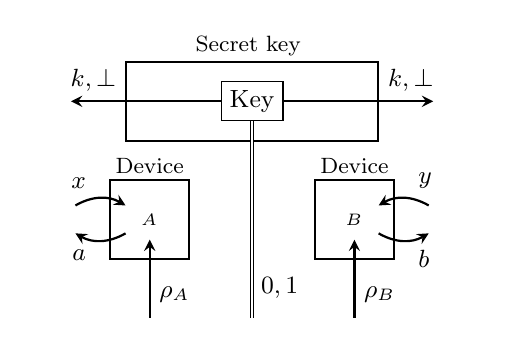
\begin{tikzpicture}[
sArrow/.style={->,>=stealth,thick},
thinResource/.style={draw,thick,minimum width=3.2cm,minimum height=1cm},
sqResource/.style={draw,thick,minimum width=1cm,minimum height=1cm},
pnode/.style={minimum width=.6cm,minimum height=.5cm}]

\small

\def\t{2.3} %1.6+.7
\def\u{.25}
\def\v{.75}
\def\w{1.3} 
\def\z{2}

\node[thinResource] (keyBox) at (0,\v) {};
\node[yshift=-1.5,above] at (keyBox.north) {\footnotesize
  Secret key $\aK$};

\node[draw] (key) at (0,\v) {Key};
\node (a1) at (-\t,\v) {};
\node (b1) at (\t,\v) {};
\node (eve) at (0,-\z) {};

\draw[sArrow] (key) to node[pos=.85,auto] {$k,\bot$} (b1.center);
\draw[sArrow] (key) to node[pos=.85,auto,swap] {$k,\bot$} (a1.center);
\draw[double] (eve.center) to node[pos=.15,auto,swap] {$0,1$} (key);


\node[pnode] (a2) at (-\t-\u,-\v) {};
\node[pnode] (b2) at (\t+\u,-\v) {};

\node[sqResource] (da) at (-\w,-\v) {$\aD_A$};
\node[yshift=-1.5,above] at (da.north) {\footnotesize
  Device};
\node[pnode] (dan) at (-\w,-\v) {};
\node[sqResource] (db) at (\w,-\v) {$\aD_B$};
\node[yshift=-1.5,above] at (db.north) {\footnotesize
  Device};
\node[pnode] (dbn) at (\w,-\v) {};

\node (eveq1) at (-\w,-\z) {};
\node (eveq2) at (\w,-\z) {};

\draw[sArrow] (eveq1.center) to node[pos=.3,auto,swap] {$\rho_A$} (dan);
\draw[sArrow] (eveq2.center) to node[pos=.3,auto,swap] {$\rho_B$} (dbn);

\draw[sArrow,bend left] (a2) to node[pos=.4,auto] {$x$} (dan);
\draw[sArrow,bend left] (dan) to node[pos=.6,auto] {$a$} (a2);
\draw[sArrow,bend right] (b2) to node[pos=.4,auto,swap] {$y$} (dbn);
\draw[sArrow,bend right] (dbn) to node[pos=.6,auto,swap] {$b$} (b2);

\end{tikzpicture}


\caption[Reusing devices]{\label{fig:open.di}An ideal world in which a
  secret key is produced by $\aK$ and new devices $\aD_A$ and $\aD_B$
  independent from $\aK$ are accessible to the players..}
\end{figure}

Unfortunately, no DI-QKD protocol has ever been shown to construct the
ideal system from \figref{fig:open.di} and it might well be impossible
to do so. But even if this is the case, it does not exclude that one
can construct an ideal system that is stronger than just the shared
secret key considered in \secref{sec:alternative.di}, e.g., one in
which the devices have some partial independence from the key or are
fully independent in certain contexts.\footnote{Context restricted
  composability is a promising research path for protocols that do not
  construct the desired ideal resource. Its investigation has been
  initiated in \textcite{JM18}, and is beyond the scope of this
  review.}

We note that weaker models such as measurement\-/device\-/independent
(MDI) QKD \--- see \secref{sec:alternative.semi} \--- do not
suffer from the same problem of device reuse as DI-QKD. The reason is
that in MDI-QKD one does not need to make any assumption about the
measurement devices at all (the adversary does the measurements for
the honest players), whereas in DI-QKD one has to assume that no
unauthorized information leaves the devices.

% This may be seen as a lack of composability: if one runs
% the protocol once in an isolated environment, the outcome remains
% secret, but if we consider a larger context where the device may be
% reused, some vital information may leak to the adversary.

% The security definitions used in device independent cryptography are
% inspired by their device dependent counterparts, e.g., the trace
% distance criterion. But unlike for the trace distance criterion, it
% has so far not been shown that these equations can be derived from a
% composable framework. In fact, it is not clear exactly what resources
% are constructed by these protocols. It is therefore an important open
% problem to develop such a framework, which enables a proper security
% analysis of device independent protocols.


\subsection{Computational security}
\label{sec:open.computational}

Computational security is a fairly unexplored area of quantum
cryptography. The main motivation for studying this is to achieve
results that are not possible with information\-/theoretic
security. For example, in \secref{sec:dqc} we mentioned a
computationally secure protocol for delegated quantum computation with
a classical client \cite{GV19}, which is believed not to be possible
with information\-/theoretic security~\cite{ACGK19}. The
computationally secure message transmission from
\secref{sec:computational} allows keys to be reused without the extra
communication required by QKD (\secref{sec:qkd}) or key recycling
(\secref{sec:recycle}) \--- and thus, without the possibility of an
adversary interrupting this communication and preventing the key from
being reused. And the work from \textcite{Unr13} discussed in
\secref{sec:mpc.ever} removes the need for a shared secret key in QKD
by using signature cards instead.

One may essentially analyze any area of cryptography with
computational security to study how assumptions needed for
information\-/theoretic security may be weakened in the computational
setting. There is however no single way to model computational
assumptions, and important open questions in the field are to identify
the (best) ways of doing this. Most frequently, one proves a
reduction, i.e., if some distinguisher can guess whether it is
interacting with the real or ideal system, then this distinguisher can
be used to solve some problem which is believed to be hard. In
\secref{sec:computational} we reviewed the finite reductions from
\textcite{BMPZ19}, in which the probability of a distinguisher $\fD$
distinguishing the real and ideal worlds is bounded by the probability
of this distinguisher being successfully used \--- as part of a new
distinguisher $\fD'$ \--- to distinguish a pseudo\-/random function
from a uniform random function; see also \textcite{Rog06} for a
discussion of reductions.

Another way to define computational security would be to define an
ideal resource that falls under the control of the adversary if she
can solve some problem believed to be hard (e.g., find a collision for
a hash function). This is essentially the ``identical-until-bad''
concept of \textcite{BR06}, but adapted to composable security instead of
game-based security. To the best of our knowledge, this paradigm remains
completely unexplored in quantum cryptography.

Other works such as \textcite{CCLVW17} bound adversaries by
circuit sizes. It is not clear how to model that in a finite,
composable framework, and is important open work.



\subsection{Other setup assumptions}
\label{sec:open.other}

When a security definition is considered ``not composable'', it often
has some (setup) assumption hard-coded in it, which is not present in
the obvious composable definition, and is therefore strictly
weaker. By modeling this assumption in a composable framework, one can
get another, equivalent composable definition. We illustrated this
in \secref{sec:alternative.memoryless} by explaining how a definition for QKD based on the accessible information, which is normally not composable, can be turned into a composable
one within a model where an adversary has no (long term) quantum
memory.

Similar techniques have been used by \textcite{Unr11} to obtain
commitments in the bounded storage model. While it follows from
\textcite{VPdR19} that coin flipping and bit commitment are impossible
in a bounded storage model without further assumptions,
\textcite{Unr11} avoids these by putting a bound on the number of
times a protocol can be run in parallel, and designing protocols that
are secure for this limited number of compositions.\footnote{This
  effectively restricts what the distinguisher/environment may do to
  distinguish the real and ideal systems, since the bound on the
  number of executions of a protocol applies to the distinguisher as
  well.} Likewise, \textcite{Pro20} has made extra setup assumptions
in the relativistic model to avoid the impossibility results of
\textcite{VPdR19}.
  
  There are numerous works where security is proved based on the assumption that adversaries are restricted. For example, adversaries cannot share entanglement in
\textcite{BCFGGOS14}, the adversaries' memory size is bounded in
\textcite{DFSS07,DFSS08}, the adversaries' memory is noisy in
\textcite{WST08,STW09,KWW12}, or adversaries can only perform local
operations on single qubits and communicate classically in
\textcite{Liu14,Liu15}. It remains open how to model these assumptions
to get composable security statements and prove in what setting such
protocols are secure. Similarly, to capture position\-/based
cryptography \textcite{Unr14} uses a model of circuits with positions in
space\-/time. Here too, it is not clear how to fit these results in a
composable framework and identify the resource that is constructed by these
protocols.


%%% Local Variables:
%%% TeX-master: "main.tex"
%%% End:
